\documentclass[11pt]{article}

%---------------------------------------------------------------------------------------------------------------------------------------------
% Mesh Data structure 
%                                          
%---------------------------------------------------------------------------------------------------------------------------------------------

\usepackage{amsmath,amssymb}
\usepackage{graphicx}
\usepackage{verbatim}
\usepackage{bm}
\usepackage{epstopdf,epsfig}

\usepackage{multirow}
\usepackage{array}
\usepackage{hhline}


\graphicspath{{figs/}}


\setlength{\textwidth}{6.5in}  \setlength{\textheight}{9.0in}   %
\setlength{\oddsidemargin}{0in} \setlength{\evensidemargin}{0in} \setlength{\topmargin}{-0.5in}  
\parskip=5pt

\renewcommand{\labelenumii}{\alph{enumii}.}
\renewcommand{\labelenumi}{\textbf{\arabic{enumi})}}

\newcommand{\bmatc}{\left[\begin{array}{c}}
\newcommand{\bmatcc}{\left[\begin{array}{cc}}
\newcommand{\bmatccc}{\left[\begin{array}{ccc}}
\newcommand{\emat}{\end{array}\right]}

\newcommand{\pd}[2]{\frac{\partial #1}{\partial #2}}
\newcommand{\pdd}[2]{\frac{\partial^{2} #1}{\partial #2^{2}}}
\newcommand\dd[2]{\ensuremath{\frac{d #1}{d #2}}}

\newcommand\vbtim[1]{\begin{verbatim} #1 \end{verbatim}}

\title{The 2DG Code \\ \small{version 4.0}}

\date{}

\begin{document}

\maketitle

\section{Data Structures}


\subsection{The \texttt{mesh} data structure}

 We will describe the  \texttt{mesh} data structure with the help of the following (coarse) triangular mesh for the unit circle:
 
\begin{figure}[h]	
\begin{center}
	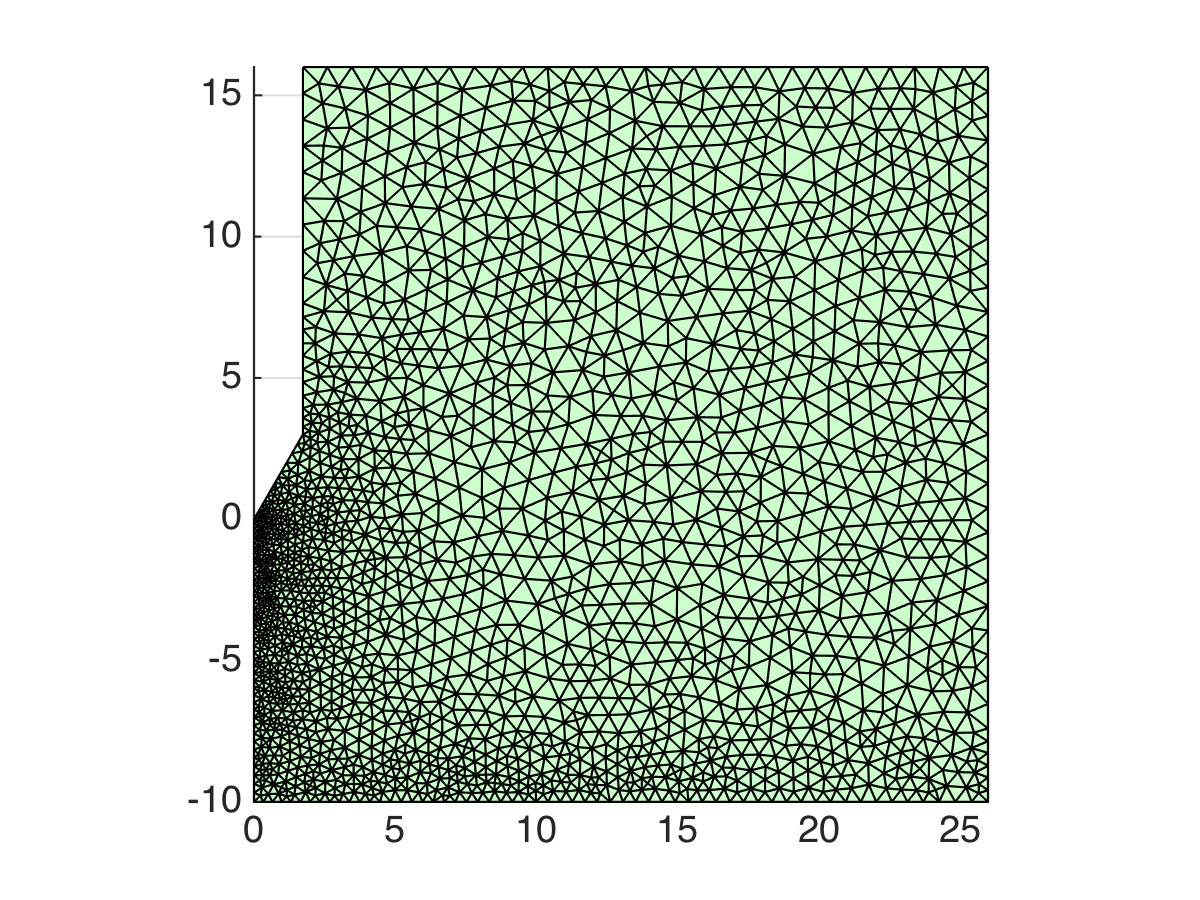
\includegraphics[scale=0.4]{mesh.png} 
	\end{center}
		\caption{Example of a triangular mesh}
		 \label{meshlinear}
	\end{figure}

The  \texttt{mesh} data structure contains the following information:

\begin{itemize}

\item {\bf The triangular linear mesh.} This mesh consists of \texttt{np} vertices and \texttt{nt} triangles. For the example in figure \ref{meshlinear} we have 
\texttt{np = 9} and \texttt{nt = 9}.

\begin{tabular}{|ll}
       	\texttt{mesh.p[np,2]}: & \texttt{x} and \texttt{y} coordinates of vertices in triangulation for simplicial mesh\\  \\ 
	
	 \multicolumn{2}{|l}{ \includegraphics[scale=0.5]{meshp}} \\
	 
	\texttt{mesh.t[nt,3]}: & Element vertices for simplicial mesh (numbered counterclockwise) \\  \\
	
	 \multicolumn{2}{|l}{ \includegraphics[scale=0.5]{mesht}}
\end{tabular}
\item {\bf Face and element connectivity information.} Here, \texttt{nf} is the number of faces (or edges in 2D) and can be calculated as
\texttt{nf  =  (3*nt + nb)/2}, where \texttt{nb} is the number of boundary edges. For our example \texttt{nb = 7}, so \texttt{nf = 17}.
We introduce two arrays: \texttt{mesh.f[nf,4]} and \texttt{mesh.t2f[nt,3]}. 

\begin{figure}[h]	
\begin{center}
	\includegraphics[scale=0.8]{face} 
	\end{center}
		\caption{Definition of an interior face \texttt{if} (left), and a boundary face  \texttt{if} on  boundary \texttt{ib}. }
\end{figure}


A face  is defined as the segment joining two vertices in the triangular mesh. \texttt{mesh.f(:,1:2)} are the indices of the two vertices in the mesh.
\texttt{mesh.f(:,3)} is the index of the triangle
	to the left of the edge (when walking from  \texttt{mesh.f(:,1)}  to  \texttt{mesh.f(:,2))}. For interior edges \texttt{mesh.f(:,4)} is the index of the triangle
	to the right of the edge. In addition, interior edges are always oriented so that  \texttt{mesh.f(:,1) < mesh.f(:,2)}. For boundary edges \texttt{mesh.f(:,4)} is the \emph{negative} of the boundary indicator. For the case of the circle we only have one boundary type and hence for these edges  \texttt{mesh.f(:,4) = -1}. Note that this convention implies that all the boundary edges are oriented counterclockwise.  Finally, for computational efficiency, the edges are ordered so that all interior edges are
	placed first and the boundary edges are last in the edge list. \\ \\ 
	


\begin{tabular}{|ll}

       	\texttt{mesh.f[nf,4]}: & \texttt{mesh.f(:,1:2)} are the indices of the two vertices in the mesh. \\ &   \texttt{mesh.f(:,3)}  is the index of the triangle
	to the left of the edge  \\ &  (when  walking from    \texttt{mesh.f(:,1)}  to  \texttt{mesh.f(:,2)}). Note that \\ & all boundary edges are last and that for all the interior
	edges  \\ & \texttt{mesh.f(:,1) < mesh.f(:,2)}.\\ \\
	
	  \multicolumn{2}{|l}{\includegraphics[scale=0.5]{meshf}} \\
	 
	  \multicolumn{2}{|l}{For this example there is only one geometric boundary \texttt{ib =  -1}.} \\  \\

	\texttt{mesh.t2f[nt,3]}: & Triangle to face connectivity. \texttt{mesh.t2f[it,in]} contains the  face \\ & number in element \texttt{it} which is opposite node \texttt{in} of element  \texttt{it}. \\ &  If the face orientation matches the element counterclockwise  \\ & orientation then the face 
	number is stored,
	otherwise the negative  \\ & of the face number is stored. \\  \\
	
	  \multicolumn{2}{|l}{\includegraphics[scale=0.5]{mesht2f}} \\

\end{tabular} 

\newpage 

\item {\bf Geometry information}

\begin{tabular}{|ll}
%      	\texttt{mesh.fd}: & Pointer to boundary distance function. The first argument to the   \\   &  the function is an array containing the
%	point coordinates given as   \\    &   \texttt{p(:,2)}.  Additional arguments can be given in \texttt{mesh.fdargs}.  The \\ & function returns
%	 the distance to the closest point on the boundary. \\ & (\texttt{mesh.fd} \emph{ can be the same function used in the }
%	  \texttt{Distmesh2D} \emph{mesh }
%	 \\ &     \emph{ generator}). \\ \\
	 
%	 \multicolumn{2}{|l}{ \includegraphics[scale=0.5]{meshfd}} \\

%	\texttt{mesh.fdargs}: & List of additional arguments for the function \texttt{mesh.fd}  \\ \\
	
%	  \includegraphics[scale=0.5]{meshfdargs} \\
	  
%	    \multicolumn{2}{|l}{For this example no additional arguments are required.} \\  \\
	  
       \texttt{mesh.fcurved[nf]}: & Logical flag indicating which faces are curved. This flag should also  \\ &  be active for straight faces with non-constatn Jacobian.\\ \\
       
        \multicolumn{2}{|l}{ \includegraphics[scale=0.5]{meshfcurved}} \\
        
       \texttt{mesh.tcurved[nt]}: & Logical flag indicating which triangles  have at least a curved \\ &  face. This flag should also be active for
       non curved triangles with \\ & non-constant Jacobian. \\   \\
              
        \multicolumn{2}{|l}{ \includegraphics[scale=0.5]{meshtcurved}} \\
        
\end{tabular}

\newpage 

\item {\bf Master Element information}

\begin{tabular}{|ll}
        \texttt{mesh.porder}: & Order of the complete polynomial used for approximation inside each element. \\  \\
        
        \multicolumn{2}{|l}{ \includegraphics[scale=0.5]{meshporder}} \\
        
	\texttt{mesh.plocal[npl,3]}: & Parametric coordinates of the nodes in the master element. Note that  \\ 
	& \texttt{mesh.plocal(:,1) = 1-mesh.plocal(:,2)-mesh.plocal(:,3)}. Also, \\ & \texttt{npl = (mesh.porder+1)*(mesh.porder+2)/2}. The order 
	of the nodes \\ &  is that shown  in figure \ref{masterel}. \\ \\
		 
	  \multicolumn{2}{|l}{ \includegraphics[scale=0.5]{meshplocal}} \\
	  
	\texttt{mesh.tlocal[ntl,3]}: & Element vertices for local auxiliary mesh. The element ordering is \\ & arbitrary. (Used for refinement and plotting). \\ \\
	
	 \multicolumn{2}{|l}{ \includegraphics[scale=0.5]{meshtlocal}} \\
\end{tabular}

\begin{figure}[h]
\begin{center}
	\includegraphics[scale=0.3]{master}  
	\end{center}
			\caption{Node positions in master element and local auxiliary mesh connectivity.  }
			\label{masterel}
\end{figure}

\item {\bf FEM node locations}

\begin{tabular}{|ll}
 \texttt{mesh.dgnodes[npl,2,nt]}: & \texttt{mesh.dgnodes[ipl,1:2,it]} are the \texttt{x} and \texttt{y} coordinates of the \\ & \texttt{ipl} local node in element \texttt{it}. Note that the nodes that lie on a \\ & curved boundary must be placed on the actual geometry as shown \\ &  in figure \ref{meshdgnodes}. \\
 \end{tabular}
\end{itemize}
 
 \begin{figure}[h]	
\begin{center}
	\includegraphics[scale=0.4]{meshdg}
	\end{center}
		\caption{DG node placement for curved geometries.  }
		\label{meshdgnodes}
\end{figure}
 
 \newpage
 
\subsection{The \texttt{master} data structure}

The \texttt{master} data structure contains master element pre-computed information such as  the parameters
required for numerical integration, the value of the shape functions and their derivatives as well as connectivity information required for efficient assembly.


\begin{itemize}

\item {\bf Master Element information}

{The variable \texttt{master.porder = mesh.porder} and the array \texttt{master.plocal = mesh.plocal} are duplicated for convenience.}

\bigskip

\begin{tabular}{|ll}
        \texttt{master.porder}: & Order of the complete polynomial used for approximation inside \\ &  each element. \\  
            \\ 
	\texttt{master.plocal[npl,3]}: & Parametric coordinates of the nodes in the master element. \\	 \\
	
	\texttt{master.ploc1d[npl1d,3]}: & Parametric coordinates for the 1D master element. Here, \\ & \texttt{npl1d = master.porder+1} \\	 
	
     \multicolumn{2}{|l}{ \includegraphics[scale=0.5]{masterloc1d}} \\
\end{tabular}


 \begin{figure}[h]	
\begin{center}
	\includegraphics[scale=0.4]{masternodes}
	\end{center}
		\caption{Local node numbering for a cubic triangular element.  }
		\label{masternodeslab}
\end{figure}

\newpage 

\item {\bf Node Templates}

\begin{tabular}{|ll}
        \texttt{master.corner[3]}: & Node numbers of the three corner nodes (see figure \ref{masternodeslab}). \\  
             \multicolumn{2}{|l}{ \includegraphics[scale=0.5]{mastercorner}} \\
            \\ 
		\texttt{master.perm[npl1d,3,2]}: & Nodes numbers of the nodes on each edge. Note that, \\ &  \texttt{npl1d = master.porder+1}. 
		\texttt{master.perm[:,ifl,1]} is the \\  & list of nodes on face \texttt{ifl} taken clockwise and \texttt{master.perm[:,ifl,2]} \\ & is the list of
		 nodes on face \texttt{ifl} taken counterclockwise (see figure \ref{masternodeslab}).  \\
			 
	 \multicolumn{2}{|l}{ \includegraphics[scale=0.5]{masterperm}} \

\end{tabular}

\bigskip

\item {\bf Numerical Integration}

\begin{tabular}{|ll}
        \texttt{master.gpts[ng,2]}: & Parametric coordinates $\{(\xi, \eta) \ | \ \xi \ge 0, \ \eta \ge 0, \ 1-\xi-\eta \ge 0 \}$ of the integration \\ & points in 2d. Here, \texttt{ng} is the number of 2D integration points.  \\  
            \\ 
        \texttt{master.gwgh[ng]}: & Integration weights in 2D. \\
           \\
         \texttt{master.gp1d[ng1d]}: & Parametric coordinates $\{\xi \ | \ \xi \ge 0, \ \xi \le 1 \}$ of the integration points in 1d. \\ & Here, \texttt{ng} is the number of 1D integration points.             \\  \\ 
        \texttt{master.gw1d[ng1d]}: & Integration weights in 1D. \\
\end{tabular}

\bigskip

\item {\bf Shape Functions}

\begin{tabular}{|ll}
        \texttt{master.shap[npl,3,ng]}: & Value of the 2D cardinal (or nodal) shape functions and their \\ & derivatives  evaluated at the integration points. Here,  \\ & \texttt{master.shap[npl,1,ng]}  contains the value of the shape function \\ & and  \texttt{master.shap[npl,2:3,ng]}  contains the values of the
        derivatives \\ & of the shape functions with respect  to  $\xi$ and $\eta$. 
            \\  \\ 
       \texttt{master.sh1d[npl1d,2,ng1d]}: & Value of the 1D cardinal (or nodal) shape functions and their \\ & derivatives evaluated at the integration points. Here, \\ &  \texttt{master.sh1d[npl1d,1,ng1d]}   contains the value of the shape \\ &  function and  \texttt{master.sh1d[npl1d,2,ng1d]}  contains the values of \\ & the
        derivatives of  the shape functions with respec  to  $\xi$. 
\end{tabular}

\newpage

\item {\bf Pre-computed Element Matrices}

\begin{tabular}{|ll}
        \texttt{master.mass[npl,npl]}: &  Mass matrix in 2D. The entry \texttt{master.mass[i,j]} corresponds \\ & to
        $ \int_{K'} \phi_i \phi_j \, d K' $, where $K'$ is the master element
            \\  \\ 
        \texttt{master.conv[npl,npl,2]}: &  Convection matrices in 2D. The entry \texttt{master.conv[i,j,1]} \\ & corresponds  to
        $ \int_{K'} \phi_i \phi_{j,\xi} \, d K' $, whereas  \texttt{master.conv[i,j,2]} \\ & corresponds to $ \int_{K'} \phi_i \phi_{j,\eta} \, d K' $.
%            \\  \\ 
%       \texttt{master.ma1d[npl1d,npl1d]}: & Mass matrix in 1D. The entry \texttt{master.ma1d[i,j]} corresponds \\ & to
 %       $ \int_{K'_{1d}} \phi_i \phi_j \, d K_{1d}' $, where $K_{1d}'$ is the 1D master element.
\end{tabular}

\end{itemize}
\newpage

\subsection{The \texttt{app} data structure}

The \texttt{app} data structure contains information regarding the application. In particular, it specifies the  equations to be solved
by providing pointers to the flux functions, but it also contains control parameters as well as the  data and the arguments necessary to evaluate the equation
fluxes. The \texttt{app} data structure can be assembled by hand for simple applications or created by a \texttt{mkapp} function.

\begin{itemize}

\item {\bf Control parameters}

\bigskip

\begin{tabular}{|ll}
        \texttt{app.nc}: & Number of components in the vector of unknowns. For scalar equations \texttt{app.nc = 1}. 
            \\ 
	\texttt{app.pg}: & Logical flag which must be set to \texttt{true} when it is necessary for the flux functions  \\
	                         & to have access to the \texttt{x} and \texttt{y} coordinates in order to evaluate the fluxes. Setting it \\
	                         & to \texttt{false} avoids costly interpolation and this should be the choice when the fluxes \\
	                         & are independent of the spatial coordinates.
	                         \\
	 \texttt{app.arg}:  & Arguments to be passed to the flux functions \texttt{app.finvi}, \texttt{app.finvb} and \texttt{app.finvv} \\
	                           & below.  \texttt{app.arg} is a cell array and can contain arrays, pointers to functions, etc. in its entries.            
\end{tabular}


\item {\bf Boundary Conditions}

\bigskip

\begin{tabular}{|ll}
        \texttt{app.bcm[ngb]}: & Boundary conditions assignment. For each of the \texttt{ngb} geometric \\   
                                           & boundaries \texttt{igb}, \texttt{app.bcm[igb]} assigns the appropriate boundary  \\ 
                                           &  condition. For instance,  if we are solving an equation on a square    \\
                                          & domain, we will typically have four geometric boundaries (\texttt{ngb = 4}), \\
                                           & but we may only have two types of boundary  conditions. In this case,  \\
                                          & \texttt{app.bcm} may look like, \texttt{app.bcm = [1,1,2,1]}. Note that the \\
                                          &   geometric boundary to which a given mesh boundary  edge \texttt{if} belongs \\
                                          & is given by \texttt{-mesh.f(if,4)}.
            \\ 
	\texttt{app.bcs[nbt,app.nc]}: & Far-field states for boundary condition application. The total number \\  
	                                              & of  boundary types is given by \texttt{nbt} and this number has to be larger or \\
	                                              &  equal to the maximum in \texttt{app.bcm}. For instance, if \texttt{app.bcm = [1,1,2,1]}, \\
	                                              & \texttt{nbt} must be at least \texttt{2}, and \texttt{app.bcs[nbt,app.nc]} contains two far field  \\	                                              & states that maybe used in order to determine the boundary conditions, \\  
	                                              &  of types \texttt{1} and \texttt{2}.
	                                            	                                              
\end{tabular}

\item {\bf Function Pointers}

In order to describe the different flux functions, we write our system of conservation laws in the form
\begin{eqnarray*}
\frac{\partial { u}}{\partial t} +  \bm{\nabla} \cdot [ \bm{F}^{\rm inv}(u, \bm{x},t)  +  \bm{F}^{\rm vis}({u},\bm{q},\bm{x},t )] = & \bm{S}({u},\bm{q},\bm{x},t) ,  \\
{\bm q} - \bm{\nabla} {u} = &  \bm{0} .  \hspace{1.6cm} 
\end{eqnarray*}

\noindent
The DG variational form the first equation is

\scalebox{0.75}{\begin{minipage}{\textwidth}
\begin{eqnarray*}
\sum_{K \in {\cal T}_h} \int_K \frac{\partial { u}_h}{\partial t}  {w} \, d {\bm x} & \\  + \displaystyle \underbrace{\sum_{e \in {\cal E}_{ih}} \int_e \widehat{\bm{F}}^{\rm inv}(u_h^+,u_h^-,\bm{x},t)  \cdot  [ w] \, ds}_{ \mbox{inter-element term I}} + 
\underbrace{\sum_{e \in \partial \Omega} \int_e \widehat{\bm{F}}^{\rm inv}(u_h^+,u_b,\bm{x},t)  \cdot  [ w] \, ds}_{ \mbox{boundary term I}}  - \underbrace{\sum_{K \in {\cal T}_h} \int_K  \bm{F}^{\rm inv}(u_h,\bm{x},t)  \cdot  \bm{\nabla} w \, d {\bm x}}_{ \mbox{volume term I}} &   \\  + 
 \displaystyle \underbrace{\sum_{e \in {\cal E}_{ih}} \int_e \widehat{\bm{F}}^{\rm vis}(u_h^+,u_h^-,\bm{q}_h^+, \bm{q}_h^-,\bm{x},t )  \cdot  [ w] \, ds}_{ \mbox{inter-element term II}} +
\underbrace{\sum_{e \in \partial \Omega} \int_e \widehat{\bm{F}}^{\rm vis}(u_h^+,\bm{q}_h^+,u_b,\bm{q}_b, \bm{x},t)  \cdot  [ w] \, ds}_{ \mbox{boundary term II}}  - \underbrace{\sum_{K \in {\cal T}_h} \int_K  \bm{F}^{\rm vis}(u_h,\bm{q}_h,\bm{x},t)  \cdot  \bm{\nabla} w \, d {\bm x}}_{ \mbox{volume term II}}  & = \\ 
\underbrace{\sum_{K \in {\cal T}_h} \int_K  \bm{S}(u_h,\bm{q}_h,\bm{x},t)  w \, d {\bm x}}_{ \mbox{source term}}
\end{eqnarray*}
\end{minipage}}

whereas for the second equation we have

\hfill\scalebox{0.75}{\begin{minipage}{\textwidth}
\begin{eqnarray*} 
& \sum_{K \in {\cal T}_h} \int_K \bm{q}_h \cdot \bm{v} \, d {\bm x} =  \displaystyle \sum_{e \in {\cal E}_{ih}} \int_e {\hat{u}}_h(u_h^+, u_h^-) \, [ \bm{v}] \, ds + 
\underbrace{\sum_{e \in \partial \Omega} \int_e {\hat{u}}_h(u_h^+, u_b) \, [ \bm{v}] \, ds}_{ \mbox{boundary term III}}  - \sum_{K \in {\cal T}_h} \int_K {u}_h \bm{\nabla} \cdot \bm{v} \, d {\bm x} 
\end{eqnarray*}
\end{minipage}}

Here, we are already assuming that the numerical flux $\hat{u}$ is not a function of $\bm{q}_h$ (that is $\bm{C}_{22} = 0$).






We will then construct functions that evaluate the fluxes at the Gauss points. Note that these functions evaluate fluxes at Gauss points and are independent of the finite element
technology or algorithm i.e. interpolation, integration rules etc.

The functions are:

\begin{tabular}{|ll}
	   \texttt{app.finvi}: & Pointer to function for the evaluation of the inviscid interface flux  \\
	                           & $\hat{\bm{F}}^{\rm inv}(u_h^+,u_h^-,\bm{x},t)$ (inter-element term I) \\
	                           & \texttt{fn = app.finvi( up, um, np, p, app.arg, time)}
	                           \\
	   \texttt{app.finvb}: &  Pointer to function for the evaluation of the inviscid boundary flux \\   
	                               &  $\hat{\bm{F}}^{\rm inv}(u_h^+,u_b,\bm{x},t)$ (boundary  term I) \\                   
	                            & \texttt{fn = app.finvb( up, np, ibt, uinf, p, app.arg, time)}
	                            \\
	    \texttt{app.finvv}: &  Pointer to function for the evaluation of the inviscid volume flux\\   
	                               &  $\hat{\bm{F}}^{\rm inv}(u_h,\bm{x},t)$  (volume term I) \\  
	                                & \texttt{[fx,fy] = app.finvv( u, p, app.arg, time)}   
	                                \\
	    \texttt{app.fvisi}: & Pointer to function for the evaluation of the viscous interface flux \\
	                           &  $\hat{\bm{F}}^{\rm vis}(u_h^+, u_h^-,\bm{q}_h^+, \bm{q}_h^-,\bm{x},t)$ (inter-element term II) \\
	                           & \texttt{fn = app.fvisi( up, um, qp, qm, np, p, app.arg, time)}
	                           	   \\
	   \texttt{app.fvisb}: &  Pointer to function for the evaluation of the viscous boundary flux  \\   
	                               & $\hat{\bm{F}}^{\rm vis}(u_h^+,\bm{q}_h^+, u_b, \bm{q}_b, \bm{x},t)$ (boundary  term II) \\                   
	                            & \texttt{fn = app.fvisb( up, qp, np, ibt, uinf, p, app.arg, time)}
	                            \\
	    \texttt{app.fvisv}: &  Pointer to function for the evaluation of the viscous volume flux  \\   
	                               & $\hat{\bm{F}}^{\rm vis}(u_h,\bm{q}_h,\bm{x},t)$ (volume term II) \\  
	                                & \texttt{[fx,fy] = app.fvisv( u, q, p, app.arg, time)} 
	                               \\
	     \texttt{app.fvisubv}: &  Pointer to function for the evaluation of the boundary flux for $u$  \\   
	                               & $\hat{u}(u_h^+,u_b,\bm{x},t)$ (boundary term III) \\  
	                                & \texttt{ub = app.fvisub( up, ibt, uinf, p, app.arg, time)} 
	                               \\
	    \texttt{app.src}: &  Pointer to function for the evaluation of the source term ${\bm{S}}(u_h,\bm{q}_h,\bm{x},t)$ \\   
	                               & (source term) \\  
	                                & \texttt{sr = app.src( u, q, p, app.arg, time)}        
	\end{tabular}

\end{itemize}




\end{document}

\item {\bf Function Pointers}
\noindent
We write our system of conservation laws in the form
\begin{eqnarray*}
{\bm q} - \bm{\nabla} {u} = &  \bm{0}, \hspace{3.7cm}  \\
\frac{\partial { u}}{\partial t} +  \bm{\nabla} \cdot \bm{F}^{\rm inv}(u)  = & \bm{\nabla} \cdot \bm{F}^{\rm vis}({u},\bm{q} ) + \bm{S}({u},\bm{q})  .
\end{eqnarray*}

\noindent
The DG variational form the first equation is

\begin{eqnarray*} 
\sum_{K \in {\cal T}_h} \int_K \bm{q}_h \cdot \bm{v} \, d {\bm x} = & \displaystyle \sum_{e \in {\cal E}_{ih}} \int_e {\hat{u}}_h \, [ \bm{v}] \, ds + 
\underbrace{\sum_{e \in \partial \Omega} \int_e {\hat{u}}_h \, [ \bm{v}] \, ds}_{ \mbox{boundary term I}}  - \sum_{K \in {\cal T}_h} \int_K {u}_h \bm{\nabla} \cdot \bm{v} \, d {\bm x}
\end{eqnarray*}
whereas for the second equation we have
\begin{eqnarray*} 
\sum_{K \in {\cal T}_h} \int_K \frac{\partial { u}_h}{\partial t}  {w} \, d {\bm x} + \displaystyle \underbrace{\sum_{e \in {\cal E}_{ih}} \int_e \widehat{\bm{F}}^{\rm inv}(u_h)  \cdot  [ w] \, ds}_{ \mbox{inter-element term I}} + 
\underbrace{\sum_{e \in \partial \Omega} \int_e \widehat{\bm{F}}^{\rm inv}(u_h)  \cdot  [ w] \, ds}_{ \mbox{boundary term II}}  - \underbrace{\sum_{K \in {\cal T}_h} \int_K  \bm{F}^{\rm inv}(u_h)  \cdot  \bm{\nabla} w \, d {\bm x}}_{ \mbox{volume term I}} & =  \\
 \displaystyle \underbrace{\sum_{e \in {\cal E}_{ih}} \int_e \widehat{\bm{F}}^{\rm vis}(u_h,\bm{q}_h)  \cdot  [ w] \, ds}_{ \mbox{inter-element term II}} + 
\underbrace{\sum_{e \in \partial \Omega} \int_e \widehat{\bm{F}}^{\rm vis}(u_h,\bm{q}_h)  \cdot  [ w] \, ds}_{ \mbox{boundary term III}}  - \underbrace{\sum_{K \in {\cal T}_h} \int_K  \bm{F}^{\rm vis}(u_h,\bm{q}_h)  \cdot  \bm{\nabla} w \, d {\bm x}}_{ \mbox{volume term II}}  & \\ +
\underbrace{\sum_{K \in {\cal T}_h} \int_K  \bm{S}(u_h,\bm{q}_h)  w \, d {\bm x}}_{ \mbox{source term}}
\end{eqnarray*}

\begin{tabular}{|ll}
          \texttt{app.fuhatb}: & Pointer to function for the evaluation of  $\hat{u}_h$ at the boundary (boundary term I). \\
                                       & \texttt{ub = app.fuhatb( ul, nl, ibt, uinf)}
            \\ 
	   \texttt{app.finvi}: & Pointer to function for the evaluation of the inviscid interface flux $\hat{\bm{F}}^{\rm inv}(u_h)$ \\
	                           & (inter-element term I) \\
	                           & \texttt{fng = app.finvi( ulg, urg, nl, plg, app.arg, time)}
	                           \\
	    \texttt{app.finvb}: &  Pointer to function for the evaluation of the inviscid boundary flux $\hat{\bm{F}}^{\rm inv}(u_h)$ \\   
	                               & (boundary  term I) \\                   
	                            & \texttt{fng = app.finvb( ulg, nl, ibt, uinf plg, app.arg, time)}
	                            \\
	    \texttt{app.finvv}: &  Pointer to function for the evaluation of the inviscid volume flux $\hat{\bm{F}}^{\rm inv}(u_h)$ \\   
	                               & (volume term I) \\  
	                                & \texttt{[fgx,fgy] = app.finvv( ug, pg, app.arg, time)}          
	\end{tabular}

\end{itemize}

 we write our system of conservation laws in the form
\begin{eqnarray*}
\frac{\partial { u}}{\partial t} +  \bm{\nabla} \cdot \bm{F}^{\rm inv}(u,\bm{x},t)  = & \bm{S}(u,\bm{x},t)  ,
\end{eqnarray*}

and the corresponding DG variational as

\begin{eqnarray*} 
\sum_{K \in {\cal T}_h} \int_K \frac{\partial { u}_h}{\partial t}  {w} \, d {\bm x} + \displaystyle \underbrace{\sum_{e \in {\cal E}_{ih}} \int_e \widehat{\bm{F}}^{\rm inv}(u_h, \bm{x},t)  \cdot  [ w] \, ds}_{ \mbox{inter-element term I}} + 
\underbrace{\sum_{e \in \partial \Omega} \int_e \widehat{\bm{F}}^{\rm inv}(u_h,\bm{x},t)  \cdot  [ w] \, ds}_{ \mbox{boundary term II}} & \\ - \underbrace{\sum_{K \in {\cal T}_h} \int_K  \bm{F}^{\rm inv}(u_h,\bm{x},t)  \cdot  \bm{\nabla} w \, d {\bm x}}_{ \mbox{volume term I}}  = \underbrace{\sum_{K \in {\cal T}_h} \int_K \bm{S}(u_h,\bm{x},t) {w} \, d {\bm x}}_{\mbox{source term}}
\end{eqnarray*}


\end{document}


























\section{Functions}
\subsection{Mesh functions}

\begin{tabular}{|lll}
	\multicolumn{3}{|l}{\texttt{[mesh.p,mesh.t] = { $\langle \mbox{generatemesh}\rangle$}(meshparam)}} \\ \\
	 \multicolumn{3}{|l}{{\bf Generate linear triangular mesh}} \\ \\
	Input: &  \texttt{meshparam} & mesh generation parameters \\ \\
	Output: & \texttt{mesh.p} &  \\
		    & \texttt{mesh.t} &   \\ \\
	   Calls:  & \texttt{distmesh2d} &  (Optional) \\
	               & \texttt{fixmesh} & (Optional) \\
\end{tabular}

\bigskip
\noindent
\begin{tabular}{|lll}
	\multicolumn{3}{|l}{\texttt{[mesh.t2t,mesh.t2n] = {mkt2t}(mesh.t)}}\\  \\
	 \multicolumn{3}{|l}{{\bf Determine neighboring element connectivity.}   This function is provided with \texttt{distmesh}} \\ \\
	Input: &  \texttt{mesh.t} &  \\ \\
	Output: & \texttt{mesh.t2t}  \ \ (The corresponding entry for elements on the boundary is zero ) &  \\
		    & \texttt{mesh.t2n}  \ \  (The corresponding entry for elements on the boundary is zero )  & \\ \\
	 Calls:  & none \\
\end{tabular}

\bigskip
\noindent
\begin{tabular}{|lll}
	\multicolumn{3}{|l}{\texttt{[mesh.plocal,mesh.tlocal] = {uniformlocalpnts}(mesh.porder)}}\\  \\
	 \multicolumn{3}{|l}{{\bf Generate uniform mesh for a master triangle in parametric space}} \\ \\
	Input: &  \texttt{mesh.porder} &  \\ \\
	Output: & \texttt{mesh.plocal} &  \\
		    & \texttt{mesh.tlocal} &   \\ \\
	 Calls:  & none \\
\end{tabular}


\section{Exercises}
\begin{itemize}
\item Modify distmesh
\item Algebraic Map
\item Accuracy Test checking Jacobian
\end{itemize}
\end{document}